% =============================================================================
% Kapitel 5: Ergebnisse und Bewertung 
% =============================================================================

\chapter{Ergebnisse und Bewertung}

In diesem Kapitel werden die empirischen Messergebnisse des entwickelten LoRaWAN-Prototyps präsentiert und dokumentiert. 
Die Evaluierung gliedert sich in die funktionale Überprüfung der TTN-Infrastruktur, die kartografische Analyse der 
Funkreichweite im Berliner Stadtgebiet sowie die messtechnische Bestimmung des elektrischen Energiebedarfs im Laborbetrieb.

\section{Validierung der Netzwerkanbindung}

Vor der Durchführung der großflächigen Feldversuche im urbanen Raum wurde die grundlegende Funktionalität der 
Kommunikationsarchitektur verifiziert. Der Fokus lag hierbei auf der fehlerfreien Initiierung des \acrshort{otaa}-Aktivierungsverfahrens sowie der 
Korrektheit der empfangenen Datenpakete auf der TTN-Serverseite der Applikation.

\begin{figure}[H]
    \centering
    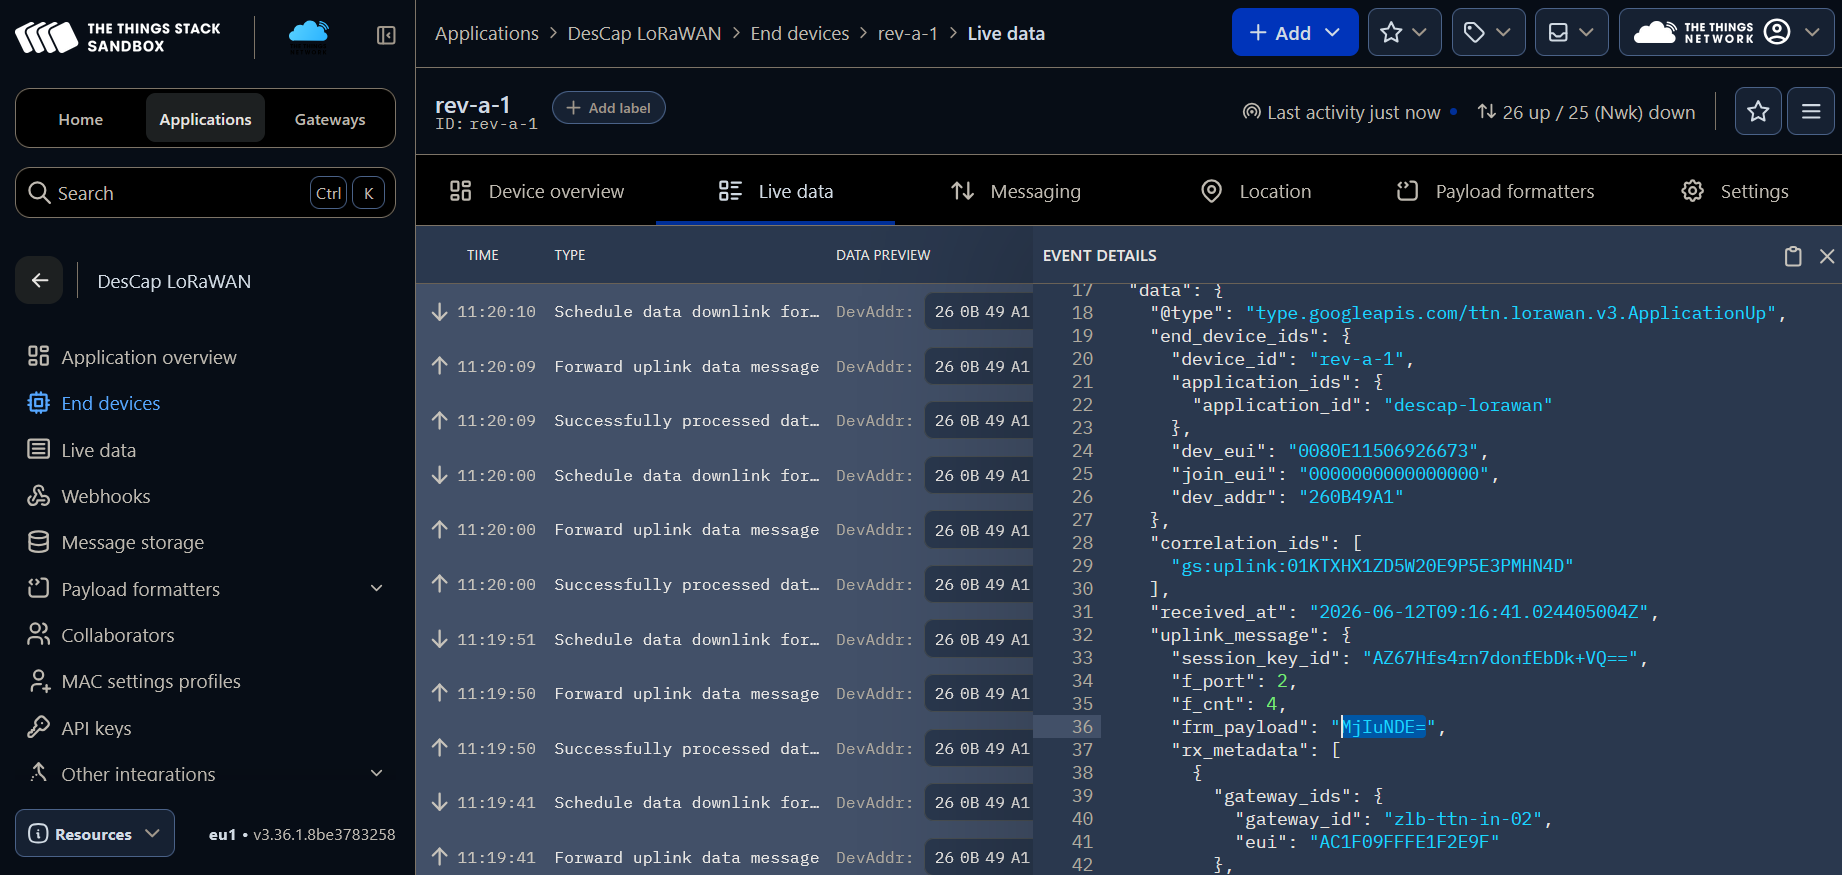
\includegraphics[width=\textwidth]{kapitel5/pictures/ttn_first_test.png}
    \caption{Screenshot von TTN-Konsole nach erfolgreichem Join-Request}
    \label{fig:ttn_first_test}
\end{figure}

Nachdem die Join-Anfrage über OTAA vom Netzwerkserver erfolgreich verarbeitet
wurde, zeigt die TTN-Konsole für das Endgerät \codebox{rev-a-1} die korrekte
DevEUI, JoinEUI sowie den Zeitstempel des Paketempfangs
an (Abbildung~\ref{fig:ttn_first_test}). Diese Übereinstimmung mit den in
der Firmware hinterlegten Werten  bestätigt, dass das Aktivierungsverfahren wie spezifiziert abgelaufen ist.

Die in Zeile 36 sichtbare Payload wird im Base64"=Format kodiert
übertragen (\codebox{MjIuNDE=}) und entspricht im Klartext dem
Temperaturwert \enquote{22.41} (\si{\celsius}). 
Anhand der in der Konsole angezeigten Gateway"=ID in Zeile 40 lässt sich das empfangende Gateway als das öffentliche
TTN"=Gateway der Zentral"= und Landesbibliothek Berlin (ZLB) identifizieren, was damit übereinstimmt, dass 
die Join"=Anfrage in unmittelbarer Nähe auf der Museumsinsel initiiert wurde. 

\section{Kartografische Evaluierung der TTN-Netzwerkabdeckung}
\label{sec:map_eval}

\begin{figure}[H]
    \centering
    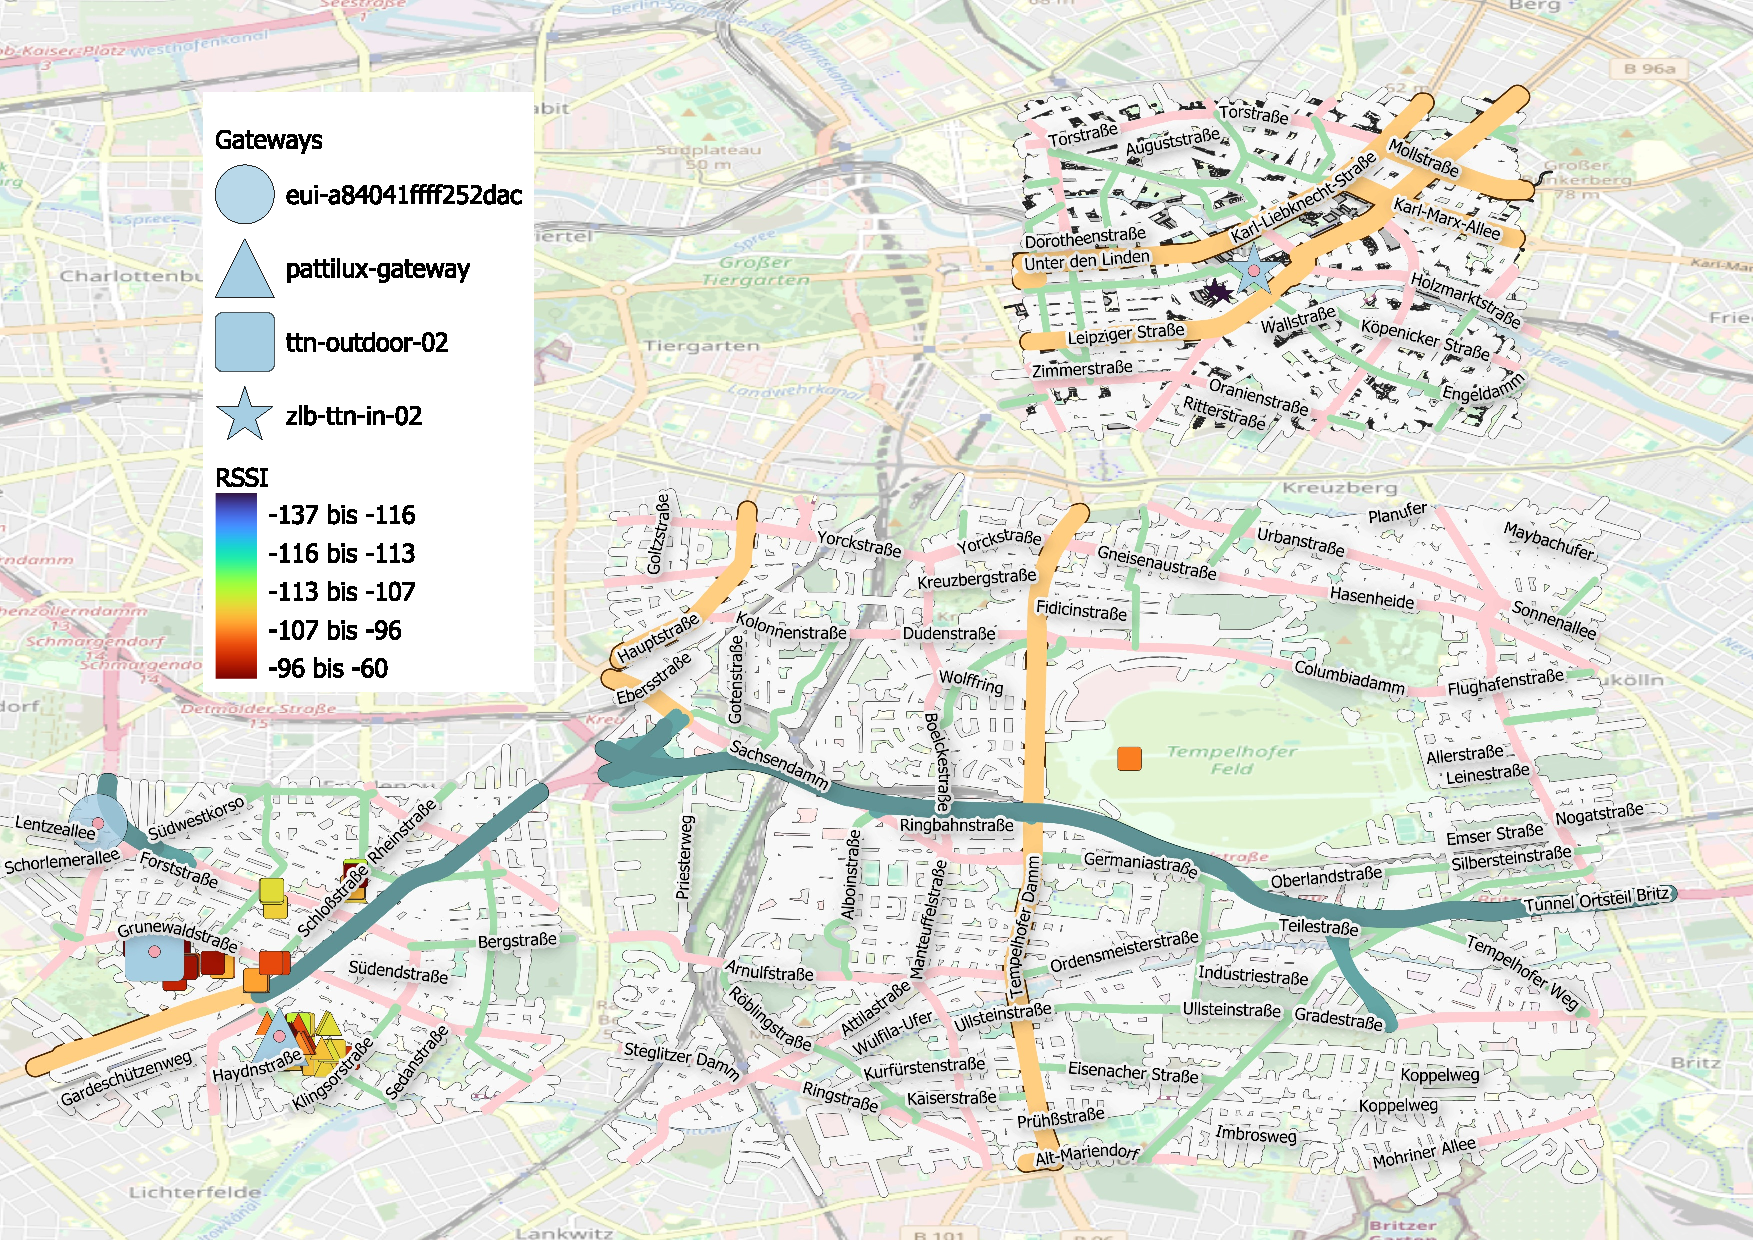
\includegraphics[width=\textwidth]{kapitel5/pictures/berlin_coverage.pdf} 
    \caption{Ergebnisse der Netzabdeckungsanalyse in Berlin.}
    \label{fig:berlin_coverage}
\end{figure}

Zur Visualisierung der Messergebnisse wurden vier ausgewählte Gateways auf der Karte hervorgehoben und in Himmelblau markiert 
Um die Gateways optisch unterscheidbar zu machen, wurde jedem eine 
eigene geometrische Form zugeordnet (Kreis, Stern, Quadrat, Dreieck). Die eigentlichen Messpunkte sind als kleinere, 
nach empfangener Signalstärke (\acrshort{rssi}) farbig kodierte Marker dargestellt. Ein Vergleich mit der öffentlich einsehbaren 
Abdeckungskarte von TTN-Mapper zeigt eine gute Übereinstimmung hinsichtlich der beobachteten RSSI-Verteilung in den untersuchten 
Stadtteilen.

\begin{figure}[H]
    \centering
    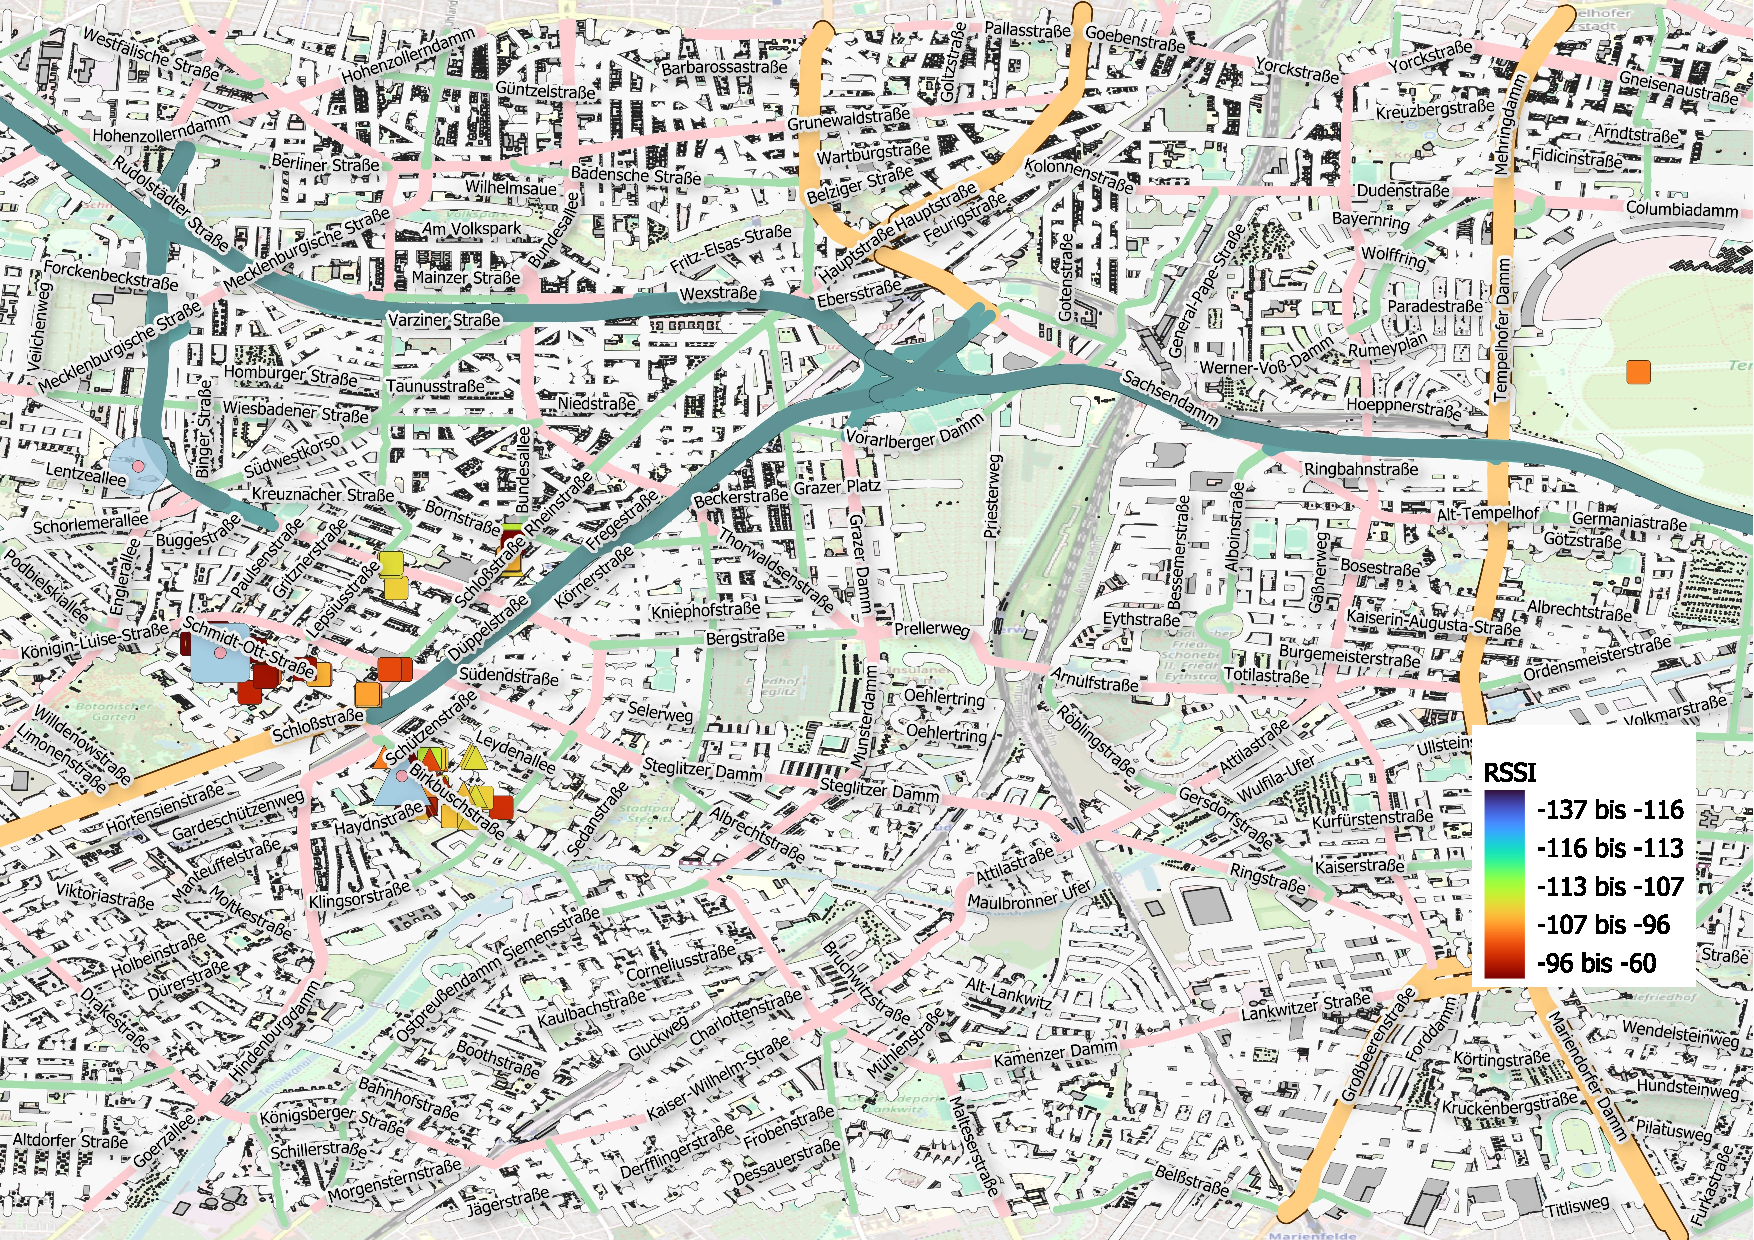
\includegraphics[width=\textwidth]{kapitel5/pictures/steglitz-tempelhof_coverage.pdf} 
    \caption{Netzabdeckungsanalyse in Steglitz und Tempelhof.}
    \label{fig:steg_tphf_coverage}
\end{figure}

Die größte gemessene Reichweite betrug rund 6 km und wurde auf dem Tempelhofer Feld vom Gateway 
in Steglitz empfangen; im unmittelbaren Steglitzer Stadtgebiet selbst lag die maximale Reichweite bei etwa 2 km. 
Von insgesamt 973 erfassten Datenpunkten trat sowohl die 2-km- als auch die 6-km-Distanz jeweils nur ein einziges Mal auf, 
was darauf hindeutet, dass derart weite Übertragungen im urbanen Raum eher die Ausnahme als die Regel darstellen. 
Die vergleichsweise große Reichweite des Gateways \codebox{ttn-outdoor-02} lässt sich durch die Antennenhöhe von rund 90 m 
über Grund erklären, die eine deutlich bessere Sichtverbindung zu entfernten Endgeräten ermöglicht als bodennahe Installationen.

\begin{figure}[H]
    \centering
    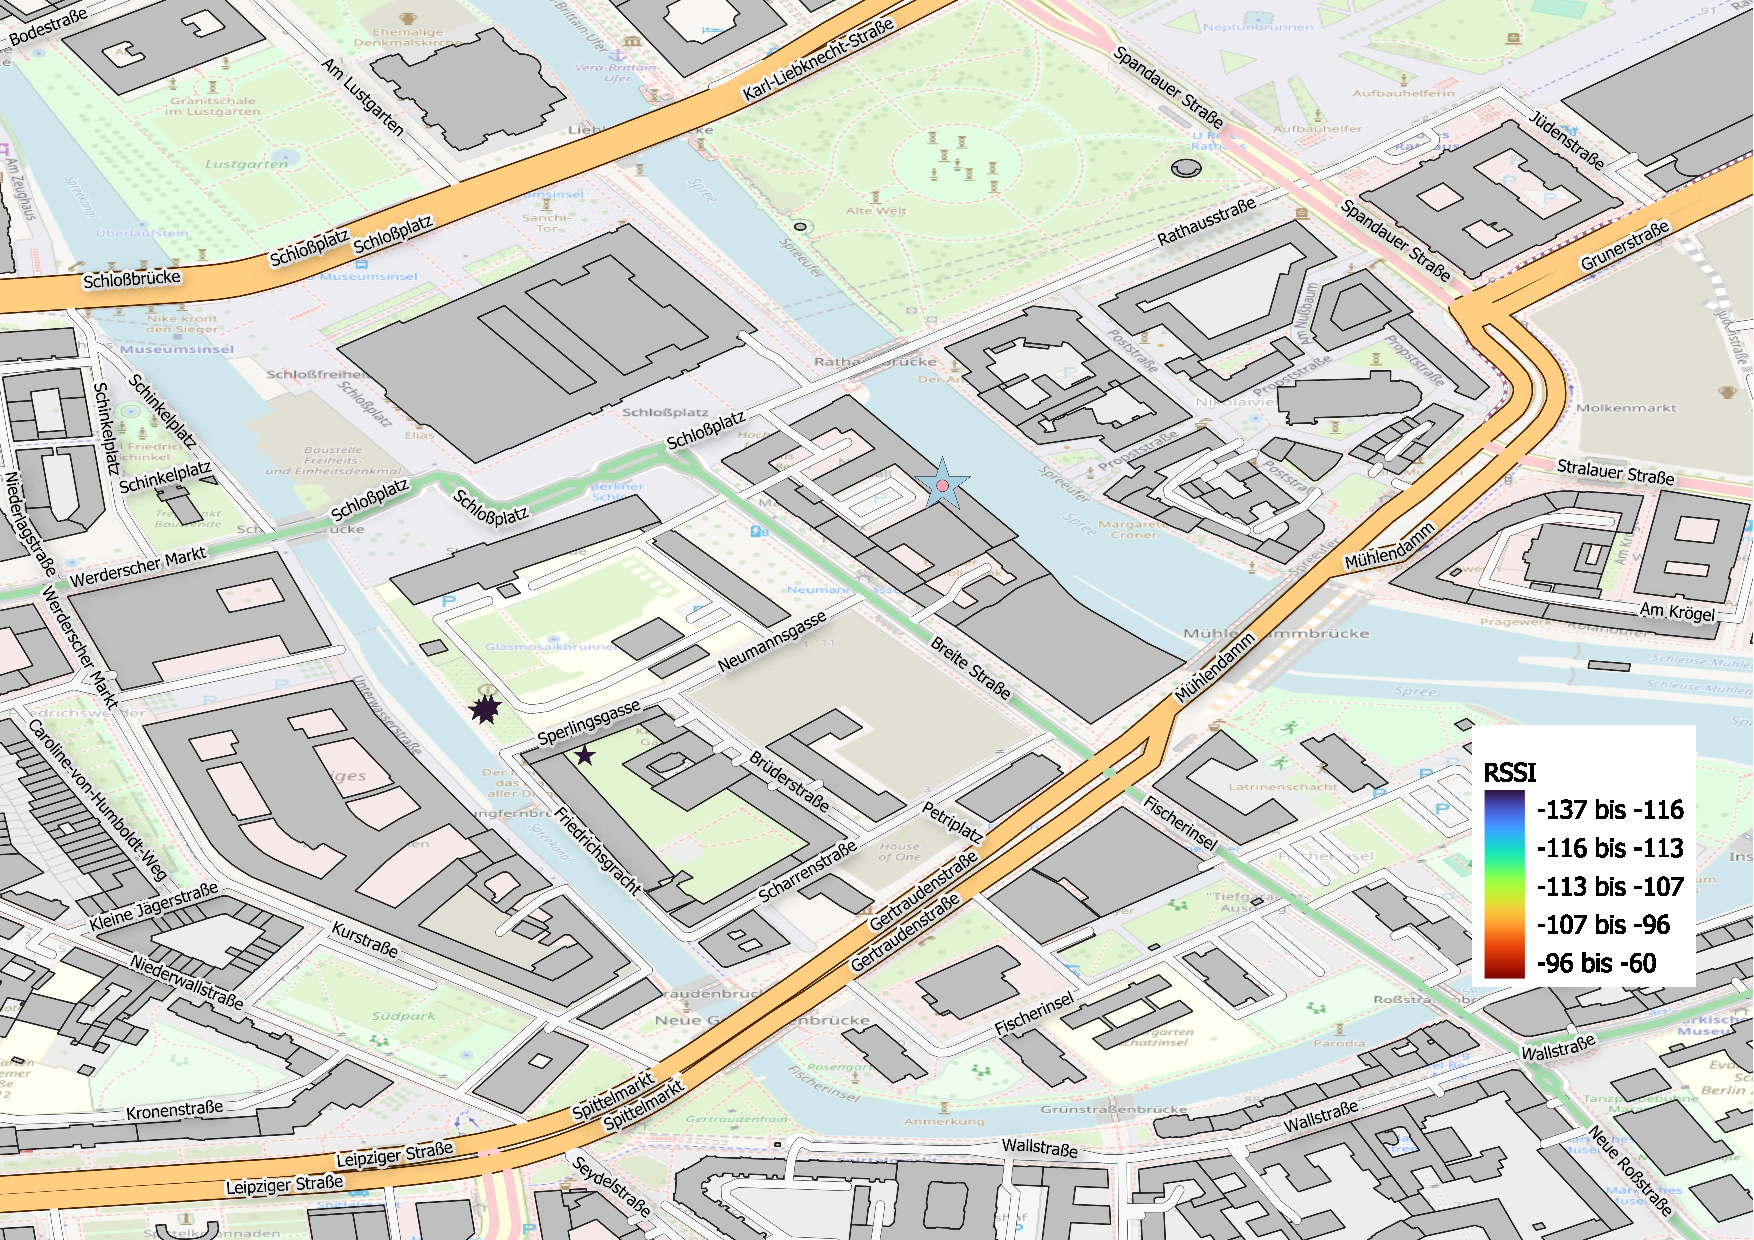
\includegraphics[width=\textwidth]{kapitel5/pictures/mitte_coverage.pdf} 
    \caption{Netzabdeckungsanalyse in Mitte}
    \label{fig:mitte_coverage}
\end{figure}

Im Gegensatz dazu fiel die reale maximale Reichweite im Bezirk Mitte mit etwa \SI{300}{\meter} deutlich geringer aus. Dies kann durch die geringe Antennenhöhe 
begründet werden, welche in diesem Fall lediglich \SI{12}{\meter} beträgt (siehe Tabelle~\ref{tab:gateway_info}). 
Die Sichtbarkeitsanalyse in Abbildung~\ref{fig:viewshed_results} deutet zwar auf eine theoretische maximale Sichtbarkeitsentfernung 
von bis zu \SI{1}{\kilo\meter} hin, diese Werte würden jedoch ausschließlich auf den Gebäudedecken der Umgebung erreicht. 
Für einen Messlauf auf Straßenhöhe resultiert daraus die Notwendigkeit, den Radius für eine zuverlässige Datenzustellung auf maximal 
\SI{300}{\meter} bis \SI{500}{\meter} um das Gateway herum zu begrenzen. Des Weiteren herrscht in den zentralen Bezirken 
Berlins eine ausgeprägte Gebäudedichte, die zu einer starken Signaldämpfung durch Absorption sowie zu häufiger Abschattung
durch topografische Sichtlinienhindernisse führt. Das Zusammenspiel dieser zwei Faktoren – Antennenhöhe und urbane Morphologie – 
rechfertigt die im Vergleich zu Steglitz bescheidenen Messergebnisse in Berlin-Mitte.

Ein technisches Problem während der Messkampagne betraf die GPS-Positionsbestimmung: Das auf der Platine verbaute L80-R-GPS-Modul 
erwies sich aufgrund einer zu langen Time-to-First-Fix als ungeeignet für den mobilen Messeinsatz, da Positionsdaten 
oft erst nach erheblicher Verzögerung (bis zu 10 Minuten) oder gar nicht zur Verfügung standen. Als Workaround wurde stattdessen eine 
GPS-Logger-App auf einem Smartphone verwendet, deren Aufzeichnungen anschließend mit den empfangenen LoRaWAN-Paketen 
zeitlich abgeglichen wurden. Insbesondere im Gebiet Mitte gingen dadurch einige Messpunkte verloren, da die GPS-Aufzeichnung 
dort zeitweise unterbrochen war.

Insgesamt zeichnen die Messergebnisse ein realistisches Bild der Funkabdeckung im städtischen Raum: Während unter günstigen 
Bedingungen -- insbesondere bei erhöhter Gateway-Antenne und freier Sichtlinie -- Reichweiten im einstelligen Kilometerbereich erreichbar sind, 
dominieren im dicht bebauten Stadtgebiet deutlich kürzere Übertragungsdistanzen.

\section{Strommessungen} 

\begin{figure}[H]
    \centering
    \begin{subfigure}[b]{\textwidth}
        \centering
        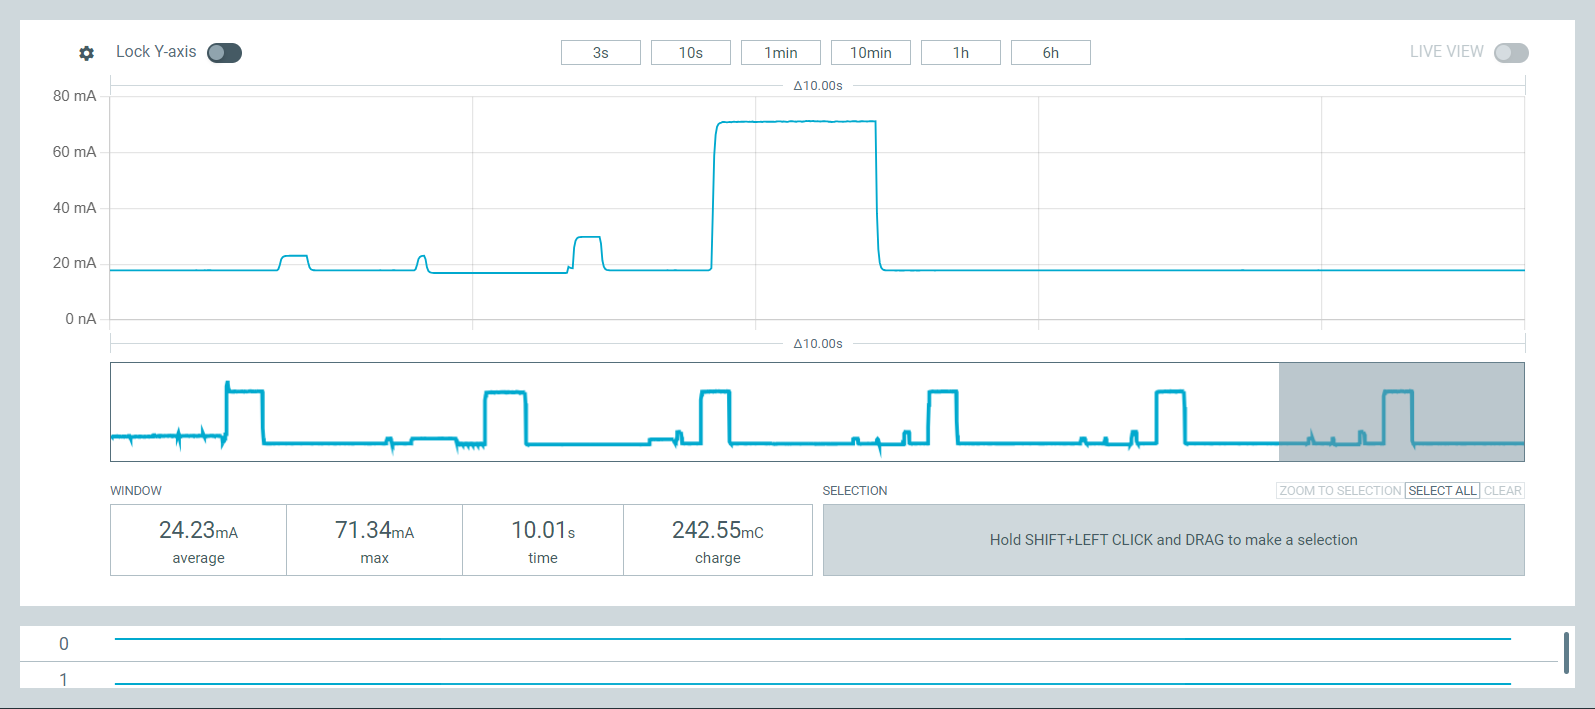
\includegraphics[width=\textwidth, height=10cm, keepaspectratio]{kapitel5/pictures/ppk2_without_bmv080.png}
        \caption{Ohne BMV080} 
        \label{fig:ppk2_1}
    \end{subfigure}
    
    \hfill
    
    \begin{subfigure}[b]{\textwidth}
        \centering
        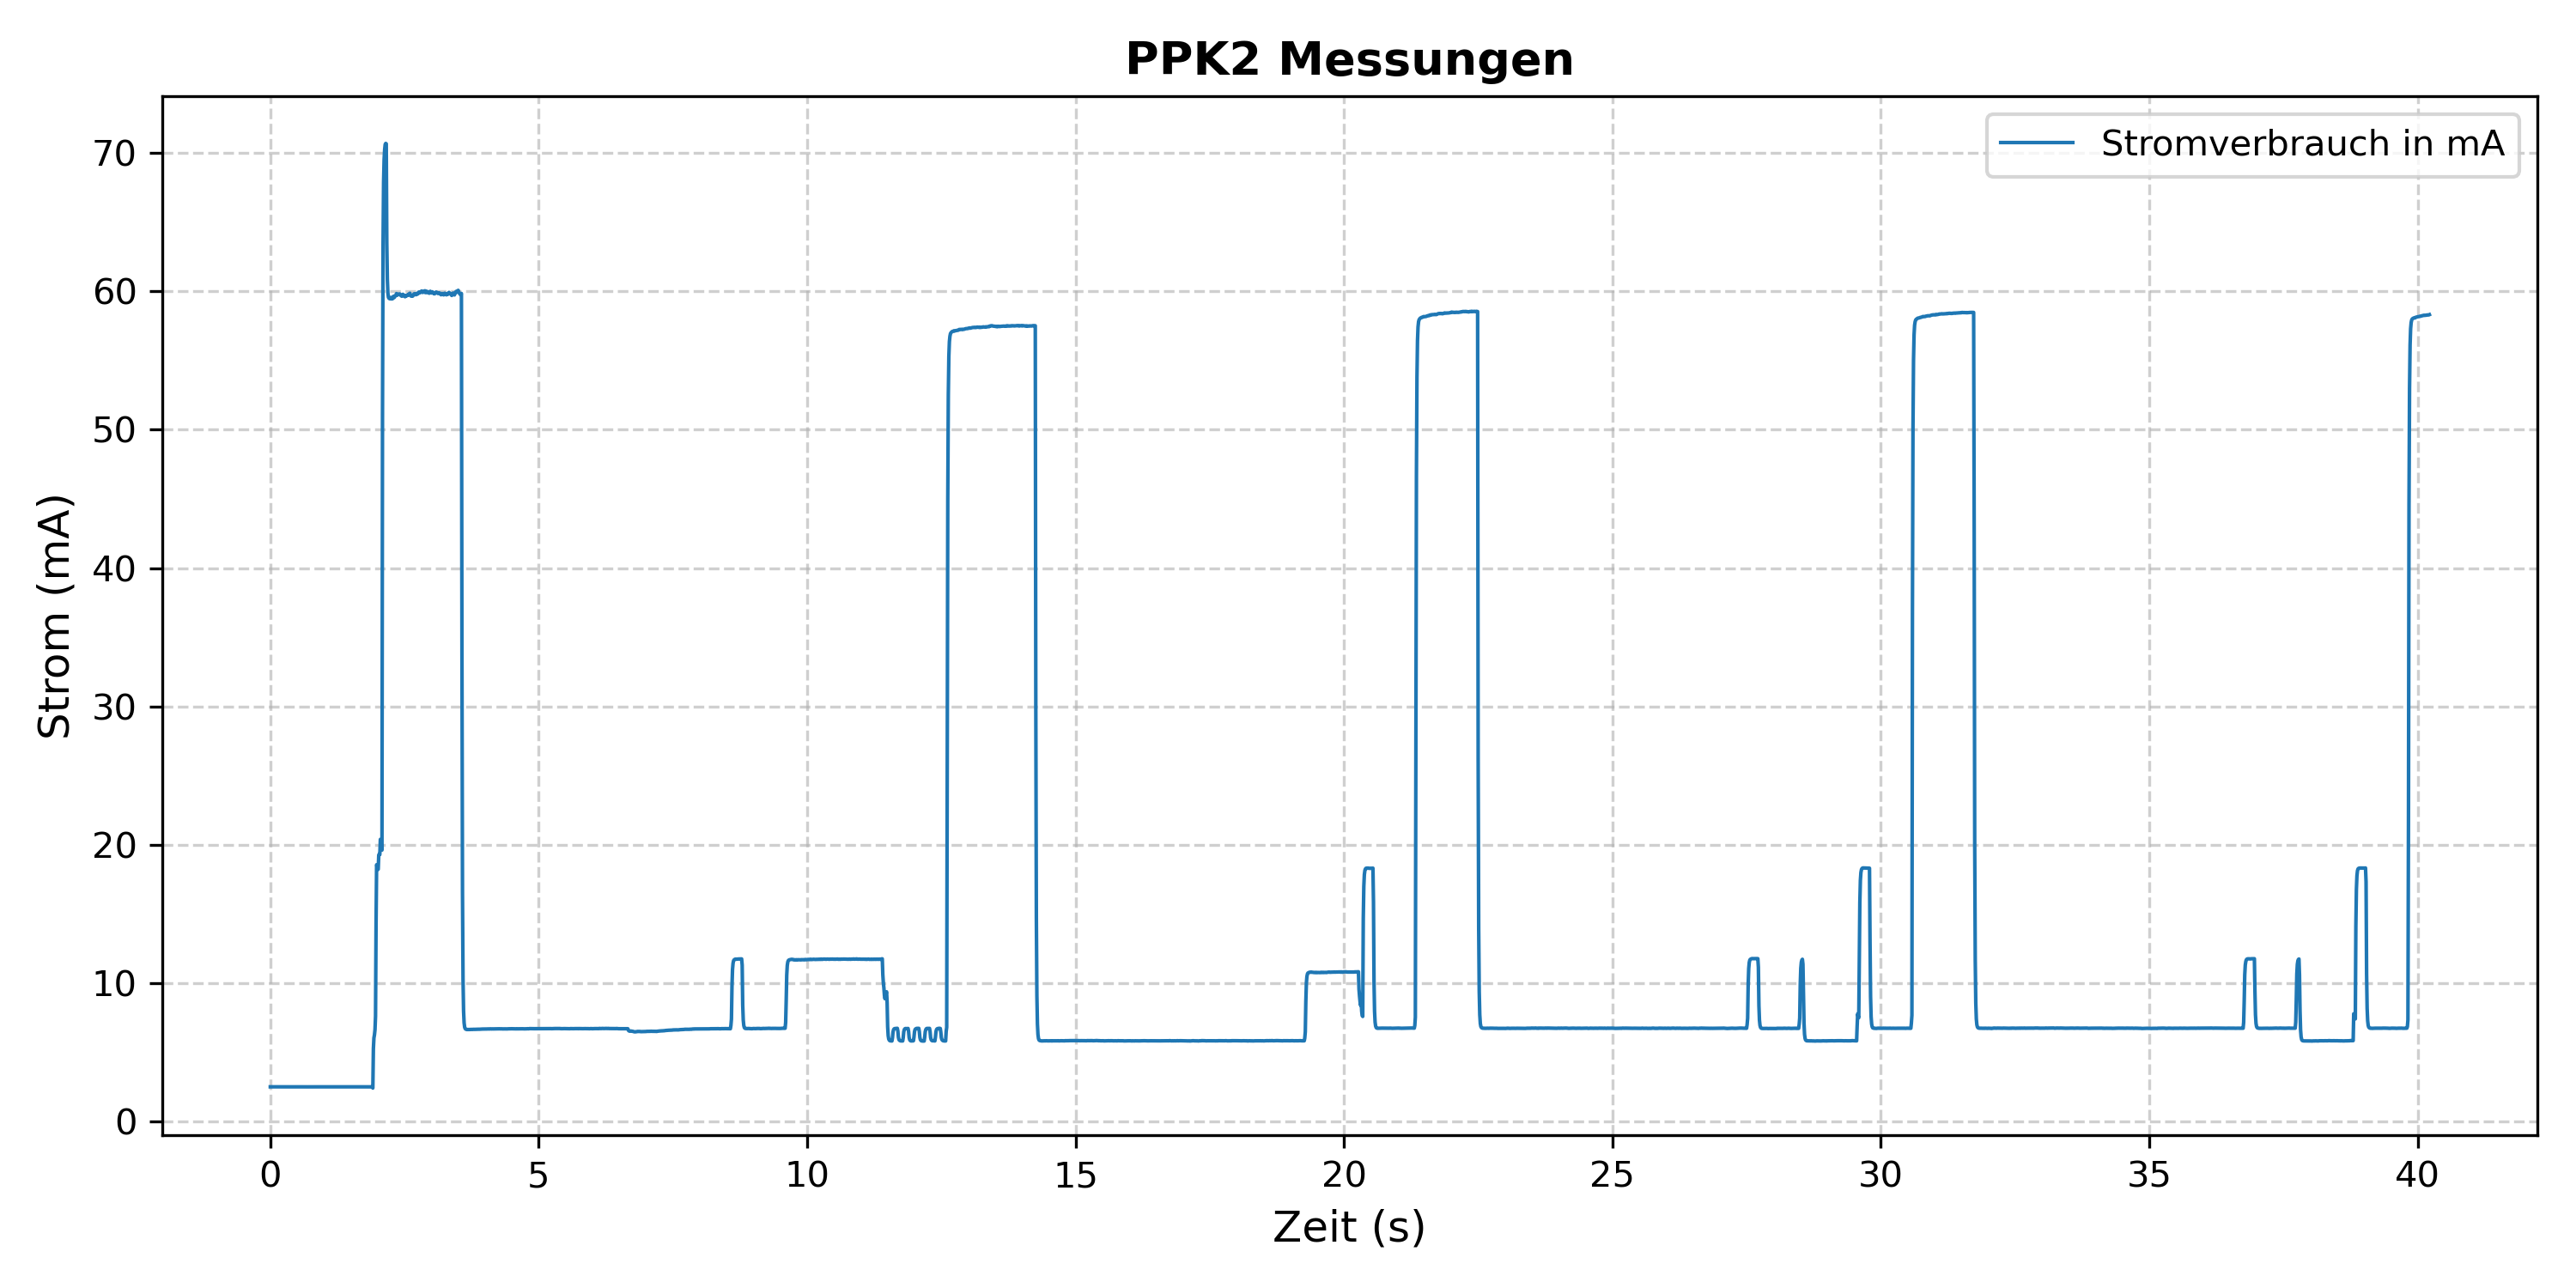
\includegraphics[width=\textwidth, height=10cm, keepaspectratio]{kapitel5/pictures/ppk2_without_gps_bmv.png}
        \caption{Ohne BMV080 und GPS} 
    \end{subfigure}
    
    \caption{Strommessungsergebnisse mit PPK2} 
    \label{fig:ppk2}
\end{figure}

Abbildung \ref{fig:ppk2} zeigt repräsentativ den Stromverbrauch des Systems, einmal mit deaktiviertem BMV080 und einmal zusätzlich
mit deaktiviertem GPS-Modul. Es lassen sich u. a. hohe Stromsprünge (auf 70 und 60 mA jeweils) in 5-Sekunden-Intervallen erkennen,
was auch der Sendehäufigkeit des Funkmoduls im Code entspricht. Der eigentliche Verbrauch des Funkmoduls ist die Amplitude des Sprungs
und beträgt jeweils $70-17=53 \text{ mA}$ und $60-3=57 \text{ mA}$ in der oberen und unteren Abbildung. Vor dem ersten Sprung
fällt ein kurzer Peak auf, der durch das Hochfahren des Funkmoduls nach einem Reset zustande kommt. 
Es ist außerdem erkennbar, wann das Endgerät mit dem OTAA-Verfahren erfolgreich aktiviert wurde, denn nach der Aktivierung soll
im Code die Status-LED 5-mal hintereinander blinken, was zu den 5 Ripple-Wellen um $t=13$ korrespondiert. 

Die Differenz von ungefähr 14 mA zwischen den zwei Abbildungen ist der Stromverbrauch des L80-R GPS-Moduls. 
Im Datenblatt des Bauteils lässt sich dieser Wert dem \emph{Acquisition-Modus} zuordnen, während dessen das Modul aktiv versucht,
erste Satelliten zu identifizieren. An dieser Stelle wird das GPS-Problem aus Abschnitt \ref{sec:map_eval} nochmal verdeutlicht:
das Modul hängt minutenlang in der Acquisition, obwohl diese maximal 30 Sekunden dauern soll. Aus diesem Grund konnten bei
Feldtests keine GPS-Daten geliefert werden. 

Ein weiteres technisches Problem wurde bei den Strommessungen offenbart: LoRa-Funktionen scheinen durch den 
Anschluss des BMV080-Partikelsensors gestört zu werden, sodass das Stromprofil des Gesamtsystems (mit allen Sensoren aktiviert)
nicht aufgezeichnet werden konnte. Es wird vermutet, dass die Ursache dieses Problems in dem Wirkprinzip des Sensors liegt.
Der BMV080 benutzt einen Laser zum Messen, welcher durch Hochfrequenz-Schaltungen erzeugt werden muss. Diese
hohen Frequenzen sowie ihre Harmoniken könnten einen erheblichen Störfaktor für das Funkmodul darstellen.
Bei künftigen Prototypen muss also der BMV080 noch mehr vom MCU getrennt werden, damit alles normal funktioniert.  

Nichtsdestotrotz lässt sich auf Basis von Abbildung \ref{fig:ppk2_1} und Tabelle \ref{tab:approx_I} der Gesamtverbrauch
auf 136,5 mA schätzen (82 mA Peak beim Hochfahren des Funkmoduls mit 54,5 mA vom BMV080). Der 200-mA-Grenzwert vom LDO des 
SPV1050-Chips (s. Kapitel \ref{chap:prot}) wird damit bei Weitem eingehalten, und nachfolgende PCB-Iterationen können
allein von der LiPo-Batterie sowie der Solarzelle versorgt werden, ohne dass ein USB-C-Ladeanschluss vorhanden sein muss.

\section{Fazit}



\section{Ausblick}

\paragraph{SPI"=Flash"=Inbetriebnahme und FUOTA}
Der auf der Platine bestückte externe SPI"=Flash"=Speicher (W25Q16JVSS)
wurde im Rahmen dieser Arbeit noch nicht aktiv genutzt. Seine Inbetriebnahme ist jedoch eine Voraussetzung für die Implementierung
von \acrfull{fuota}, die für den praktischen Einsatz in Gefahrgebieten von besonderer Relevanz ist: 
Da Endgeräte in solchen schwer zugänglichen Umgebungen nach dem Deployment häufig nicht mehr ohne erheblichen Aufwand 
physisch erreicht werden können, erlaubt FUOTA die drahtlose Aktualisierung der Firmware -- etwa zur Behebung von Fehlern, 
zur Anpassung von Betriebsparametern oder zur Erweiterung der Funktionalität -- ohne
dass ein manueller Eingriff vor Ort erforderlich ist. Aus diesem Grund bleibt die Umsetzung
Validierung des FUOTA"=Ablaufs  einer Folgearbeit vorbehalten.

\paragraph{Energieautarker Betrieb mit Solarzelle}
Das verfügt bereits über einen MPPT"=Laderegler (SPV1050), der die Anbindung eines Solarpanels ermöglicht.
Bislang wurde jedoch die LiPo-Batterie ausschließlich über den USB-C-Anschluss aufgeladen.
Die Inbetriebnahme der Solarzelle sowie eine Langzeitmessung der Energiebilanz mit dem PPK2 stellt somit 
einen sinnvollen nächsten Schritt dar, um die tatsächliche Betriebsdauer in Einsätzen zu ermitteln.

\paragraph{Antennenoptimierung}
Die verwendete Antenne wurde im Rahmen dieser Arbeit nicht messtechnisch überprüft. Eine 
Dimensionierung des Anpassnetzwerks mittels eines \acrshort{vna} (Vector Network Analyzer) wie der NanoVNA
sowie eine anschließende Strahlungscharakterisierung (Gewinn, Richtdiagramm) würden die
weitere Optimierungsmöglichkeiten offenlegen. 

\paragraph{Privates Gateway und RF"=Planung}
Die Kapitel \ref{chap:test} beschriebenen und  durchgeführten Feldversuche stützten sich ausschließlich auf öffentliche TTN"=Gateways, was sowohl die
geografische Flexibilität der Messrouten erheblich einschränkte. Eine Abwendung von TTN zugunstens der Plattform Chirpstack - 
mit der sich private LoRaWAN-Netzwerke aufbauen lassen - in Kombination mit einer gezielten RF"=Planung (mithilfe Werkzeuge wie
\href{https://github.com/UniCT-ARSLab/LWN-Simulator}{LoRaWAN-Simulator}) könnten bessere Vorhersagen bzlg. Reichweite oder
Netzabdeckung getroffen werden.

\newacronym{vna}{VNA}{Vector Network Analyzer}

